% This is samplepaper.tex, a sample chapter demonstrating the
% LLNCS macro package for Springer Computer Science proceedings;
% Version 2.20 of 2017/10/04
%
\documentclass[runningheads]{llncs}
\usepackage{hyperref}
\usepackage{xcolor}
\newcommand{\red}[1]{\textcolor{red}{#1}}
%
\usepackage{graphicx}
\usepackage{array}
% Used for displaying a sample figure. If possible, figure files should
% be included in EPS format.
%
% If you use the hyperref package, please uncomment the following line
% to display URLs in blue roman font according to Springer's eBook style:
% \renewcommand\UrlFont{\color{blue}\rmfamily}

\begin{document}
%
\title{Resolution and Optimization of a Decision Problem: C-Note}
%
\titlerunning{3MIEIC05 C-Note\_1}
% If the paper title is too long for the running head, you can set
% an abbreviated paper title here
%
\author{João Sousa \and Rafael Ribeiro}
%
\institute{FEUP-PLOG, Turma 3MIEIC05, Grupo C-Note\_1}
%
\maketitle              % typeset the header of the contribution
%
\begin{abstract}
This project, developed in the context of the curricular unit Logic Programming, using the Prolog environment SICStus, had the objective of solving a decision/optimization problem using restriction programming (SICStus' CLPFD library). The methods used to tackle this problem are described in this article.

\keywords{SICStus \and Prolog \and C-Note \and Restriction programming.}
\end{abstract}
%
%
%
\section{Introduction}
This project was developed in the context of the final project for the curricular unit Logic Programming, in the 3rd year of the Masters in Informatics and Computing Engineering. The group had to find a possible solution for a decision/optimization problem using restriction programming. From the given options, the group chose a puzzle named \href{https://erich-friedman.github.io/puzzle/100/}{C-Note}, by Erich Friedman, which consists of a square matrix of single digits such that by adding digits before or after these, the sum of all rows and columns add up to 100.
The article has the following structure:
\begin{itemize}
    \item \textbf{Problem Description:} detailed description of the problem, including all involved restrictions.
    \item \textbf{Approach:} description of modeling the problem as a Constraint Satisfaction Problem.
    \begin{itemize}
        \item \textbf{Decision Variables:} description of decision variables and respective domains, as well as their meaning in the context of the problem.
        \item \textbf{Constraints:} description of hard and soft constraints, as well as their implementation using SICStus Prolog.
    \end{itemize}
    \item \textbf{Solution Presentation:} explanation of the predicates that allow the visualization of the solution.
    \item \textbf{Experiments and Results:}
    \begin{itemize}
        \item \textbf{Dimensional Analysis:} examples of execution of the problem with different dimensions and analysis of the obtained results.
        \item \textbf{Search Strategies:} testing of different search strategies/heuristics, comparing the obtained results. 
    \end{itemize}
    \item \textbf{Conclusions and Future Work:} conclusions drawn from the project, advantages and limitations of obtained solution, aspects that can be improved.
    \item \textbf{References:} bibliographic references
    \item \textbf{Attachments: } source code, images and graphs.
\end{itemize}

\section{Problem Description}
C-Note is a grid puzzle, much like Sudoku and others of its kind, where the objective is to have all rows and columns sum up to the same integer, in this case, 100. The initial grids consist of single digits and the player must add digits to the left and right of these in order to achieve the previously referred goal. 

%\begin{table*}
%\caption{Solved puzzle example}
%\parbox{.45\linewidth}{
%\centering
%\begin{tabular}{|p{1cm}|p{1cm}|p{1cm}|}
%\hline
%8&8&4\\[5pt]
%\hline
%6&2&5\\[5pt]
%\hline
%3&6&1\\[5pt]
%\hline
%\end{tabular}
%}
%\hfill
%\parbox{.45\linewidth}{
%\centering
%\begin{tabular}{|p{1cm}|p{1cm}|p{1cm}|}
%\hline
%\red{1}8&8&\red{7}4\\[5pt]
%\hline
%6\red{9}&2\red{6}&5\\[5pt]
%\hline
%\red{1}3&\red{6}6&\red{2}1\\[5pt]
%\hline
%\end{tabular}
%}
%\end{table*}

\section{Approach}
Since the initial state of the puzzle doesn't require anything beside the values on the cells, the input was represented as a list with the values of the table in sequence

\begin{table}
    \caption{Input example}
    \centering
    \begin{tabular}{|p{1cm}|p{1cm}|p{1cm}|}
    \hline
    8&8&4\\[5pt]
    \hline
    6&2&5\\[5pt]
    \hline
    3&6&1\\[5pt]
    \hline
    \end{tabular}
\end{table}
\begin{center}
    [8, 8, 4, 6, 2, 5, 3, 6, 1]
\end{center}

\subsection{Decision Variables}
The solution of a puzzle is simply a table with the replaced values, and as such is returned as a list with the same size as the input.
\begin{table}
    \caption{Output example}
    \centering
    \begin{tabular}{|p{1cm}|p{1cm}|p{1cm}|}
    \hline
    \red{1}8&8&\red{7}4\\[5pt]
    \hline
    6\red{9}&2\red{6}&5\\[5pt]
    \hline
    \red{1}3&\red{6}6&\red{2}1\\[5pt]
    \hline
    \end{tabular}
\end{table}
\begin{center}
    [18, 8, 74, 69, 26, 5, 13, 66, 21]
\end{center}

The domain of these variables are $1..Sum-Size$, since a cell must have a number larger than 0 (e.g if the sum of a row with 3 cells is 100 and no cell can hold 0, the maximum combination is [97, 1, 1]).

\subsection{Constraints}
The representation of the problem chosen by the group only has 2 hard restrictions:

\textbf{All rows and columns sum up to 100:} Rule imposed by the game. This is assured by the predicates \verb!sum_rows(Rows, Sum)! and \verb!sum_rows(Cols, Sum)!
\begin{verbatim}
% sum_rows(+Matrix, +S)
sum_rows([], _).
sum_rows([H|T], S):-
    sum(H, #=, S), sum_rows(T, S).
\end{verbatim}

\textbf{All cells in the solution \textit{must include} the digit given in the input:} Possible solutions are found through this restriction. Since the game consists of adding digits before or after the initial digit, the final solution will always hold the input value in one of its digits. This is assured by the predicate \verb!includes_digit_list(Input, Output)!
\begin{verbatim}
% includes_digit(+Var, +Input)
includes_digit(Var, Input):-
    Var mod 10  #= Input.
includes_digit(Var, Input):-
    Var #> 0,
    Rest #= Var // 10,
    includes_digit(Rest, Input).
\end{verbatim}

\textbf{Solution must be unique:} This restriction was enforced during the generation of new puzzles, and would drastically increase the time until a valid solution was found. Since the author of the puzzle doesn't specify this as a rule (his first example doesn't obey this), the group decided to leave this feature as optional.

This was achieved with the predicate \verb!more_than_once(Goal)!, \cite{ref-more} which fails if the number of times a Goal predicate succeeds is different from 1. It avoids the program from wasting time on finding all the existing solutions of a puzzle (like it would be done by something like the \verb!findall()! predicate), when it only needs to know if there is one or more possible solutions.

\newpage
\section{Solution Presentation}
To visualize this decision problem, the program features a series of menus to lead the user to all the functionalities:
\begin{verbatim}
  /$$$$$$                      /$$   /$$  /$$$$$$  /$$$$$$$$ /$$$$$$$$
 /$$__  $$                    | $$$ | $$ /$$__  $$|__  $$__/| $$_____/
| $$  \__/                    | $$$$| $$| $$  \ $$   | $$   | $$      
| $$             /$$$$$$      | $$ $$ $$| $$  | $$   | $$   | $$$$$   
| $$            |______/      | $$  $$$$| $$  | $$   | $$   | $$__/   
| $$    $$                    | $$\  $$$| $$  | $$   | $$   | $$      
|  $$$$$$/                    | $$ \  $$|  $$$$$$/   | $$   | $$$$$$$$
 \______/                     |__/  \__/ \______/    |__/   |________/


1. Solve input puzzle
2. Generate puzzle
3. Generate puzzle with unique solution
0. Exit

:- 
\end{verbatim}

One can input an existing configuration through \textbf{option 1} (check examples \href{https://erich-friedman.github.io/puzzle/100/}{here}).
Through options \textbf{2 and 3}, the program will generate and then, if the user wishes, solve a new random puzzle. The latter restricts the generated puzzle so it has an \textbf{unique} solution.

\section{Experiments and Results}
To test the chosen approach, the group ran tests varying both dimension of the problem and the search heuristic used in labeling.

\subsection{Dimensional Analysis}
The first variable to be tested was the \textbf{size of the puzzle}, where the values ranging from 3*3 to 7*7 were used. For this, puzzles with target sum 60 were generated for each test. Default labeling options were used. Graphs for this table found in the attachments. \ref{graphSizeT} \ref{graphSizeB} \ref{graphSizeC}

\begin{table}[]
    \centering
    \caption{Varying Input Size}
    \begin{tabular}{>{\centering}p{1.5cm}|>{\centering\arraybackslash}p{1.5cm}>{\centering\arraybackslash}p{1.8cm}>{\centering\arraybackslash}p{3cm}}
    \hline
    &Time&Backtracks&Constraints created\\\hline\hline
    100&0.00&202&152\\
    150&0.02&1753&597\\
    200&0.03&2665&877\\
    250&0.04&2627&845\\
    300&0.14&7265&1741\\
    400&1.00&43848&4294\\
    500&0.79&26961&1725\\
    700&1.28&42719&2142\\
    900&2.03&512087&2119\\
    1200&47.04&2971885&202\\
    1500&33.78&1099845&7124\\\hline

    \end{tabular}
    \label{tab:size}
\end{table}

From these we extrapolate that the increases in time and backtracks are exponential while the increase in constraints seems rather erratic. This may be explained by the randomness of the generated inputs.

The other variable that was tested was the target sum of the rows and columns. Puzzles were also generated for these runs, with a size of 3*3, and default labeling options were also used. Similarly, graphs can be found in the attachments. \ref{graphSumT} \ref{graphSumB} \ref{graphSumC}

\begin{table}
    \centering
    \caption{Varying Target Sum}
    \begin{tabular}{>{\centering}p{1.5cm}|>{\centering\arraybackslash}p{1.5cm}>{\centering\arraybackslash}p{1.8cm}>{\centering\arraybackslash}p{3cm}}
        \hline
        &Time&Backtracks&Constraints created\\\hline\hline
        3&0&70&93\\
        4&0.01&2068&1481\\
        5&0.18&35773&9164\\
        6&6&12447174&7296845\\
        7&116.5&20342573&581\\
        \hline
    \end{tabular}
    \label{tab:sum}
\end{table}

\newpage
\subsection{Search Strategies}
Tests were also done in the hopes of finding the most efficient search strategy used in the labeling process, below is the table of runtimes for all combinations of arguments of the predicate \verb!labeling([], Output)!\cite{ref-labeling-opts}. The options \verb!leftmost, smallest, largest, first_fail, anti_first_fail, occurrence,! \verb!most_constrained and max_regret! control the order in which the next variable is selected for assignment and the options \verb!step, enum, bisect, middle! \verb!and median! determine the way in which choices are made for the selected variable. These tests were all run on the 4*4 puzzle \verb![5, 2, 7, 1, 7, 1, 5, 9,! \verb!8, 8, 3, 7, 5, 2, 9, 1]!, with a target sum of 100.


\begin{table}
    \centering
    \caption{Search strategies runtimes}
    \begin{tabular}{p{1.2cm}||cccccccc}
    \hline
	 &leftmost&smallest&largest&first\_fail&anti\_first\_fail&occurrence&most\_constrained&max\_regret\\[0.1cm] \hline\hline
    step&0.4&1.78&2.54&4.44&0.71&0.39&3.85&0.4\\
    enum&0.39&0.42&3.5&6.11&0.93&0.51&6.24&0.52\\
    bisect&0.32&0.84&5.26&3.17&1.76&0.33&3.09&0.32\\
    middle&0.58&0.52&4.28&7.06&33.86&0.62&7.05&0.62\\
    median&0.59&0.53&4.28&6.97&45.53&0.62&7.03&0.62\\ \hline

    \end{tabular}
    \label{tabSearch}
\end{table}

From this we conclude the most efficient combination of options is \textbf{bisect \& max\_regret}, and that the option \textbf{anti\_first\_fail} yielded the worst results.

\section{Conclusions and Future Work}
The project's goal of applying the knowledge taught in practical and theoretical PLOG classes was achieved, showing how useful restriction programming can be in some cases. 

Some of the bigger obstacles faced were "switching" from the common imperative programming paradigm to the declarative style used, as well as the implementation of some of the restrictions. The predicate \verb!includes_digit(Var, Input)! was the most challenging to crack, and was a big breakthrough in our understanding of the CLPFD library.

Our solution could be improved upon, especially when it comes to generating unique solutions, which proved to be the slowest part of the program. We are not sure if much else in terms of restrictions and labeling could be done under the rules of the existing game.

We find the project was a success in contributing positvely to our knowledge of Prolog and restriction programming, having definetly piqued our interest in this way of problem solving.
\begin{thebibliography}{8}
%\bibitem{ref_article1}
%Author, F.: Article title. Journal \textbf{2}(5), 99--110 (2016)

%\bibitem{ref_lncs1}
%Author, F., Author, S.: Title of a proceedings paper. In: Editor,
%F., Editor, S. (eds.) CONFERENCE 2016, LNCS, vol. 9999, pp. 1--13.
%Springer, Heidelberg (2016). \doi{10.10007/1234567890}

%\bibitem{ref_book1}
%Author, F., Author, S., Author, T.: Book title. 2nd edn. Publisher,
%Location (1999)

%\bibitem{ref_proc1}
%Author, A.-B.: Contribution title. In: 9th International Proceedings
%on Proceedings, pp. 1--2. Publisher, Location (2010)

%\bibitem{ref_url1}
%LNCS Homepage, \url{http://www.springer.com/lncs}. Last accessed 4
%Oct 2017

\bibitem{ref-labeling-opts}
SICStus Documentation v.latest4 \url{https://sicstus.sics.se/sicstus/docs/latest4/html/sicstus.html/Enumeration-Predicates.html}

\bibitem{ref-more}
Ulrich Neumerkel, Institut für Information Systems Engineering, Wien Austria Europe
\url{http://www.complang.tuwien.ac.at/ulrich/sicstus-prolog/call_nth.pl}

\end{thebibliography}

\newpage
\section{Attachments}

\begin{figure}
    \centering
    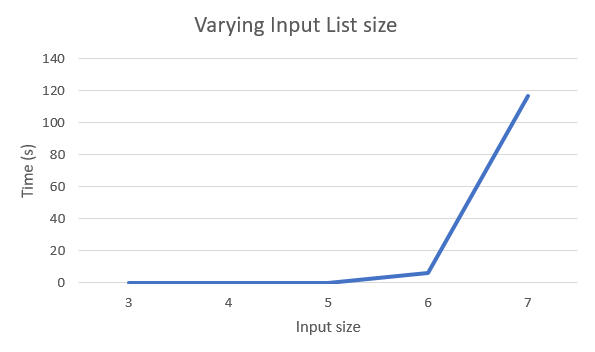
\includegraphics[width=0.8\textwidth]{graph_size_time.png}
    \caption{Graph for varying input size and time}
    \label{graphSizeT}
\end{figure}

\begin{figure}
    \centering
    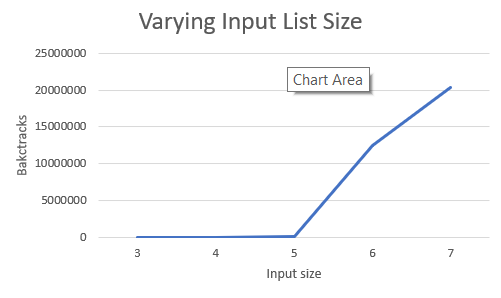
\includegraphics[width=0.8\textwidth]{graph_size_backs.png}
    \caption{Graph for varying input size and number of backtracks}
    \label{graphSizeB}
\end{figure}

\begin{figure}
    \centering
    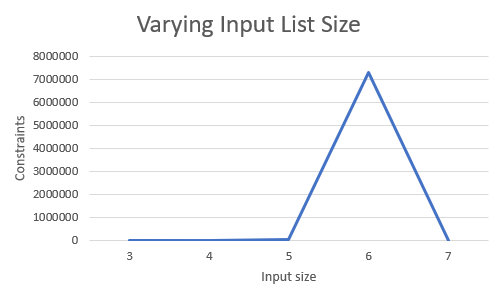
\includegraphics[width=0.8\textwidth]{graph_size_consts.png}
    \caption{Graph for varying input size and number of constraints}
    \label{graphSizeC}
\end{figure}

\begin{figure}
    \centering
    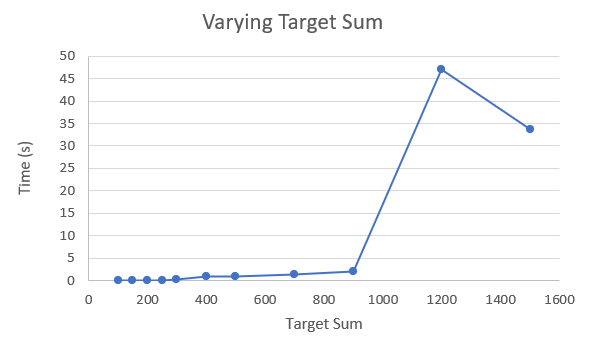
\includegraphics[width=0.8\textwidth]{graph_sum_time.png}
    \caption{Graph for varying target sum and time}
    \label{graphSumT}
\end{figure}

\begin{figure}
    \centering
    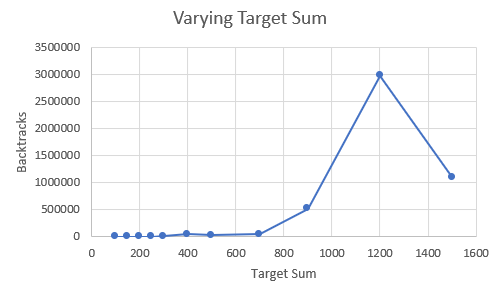
\includegraphics[width=0.8\textwidth]{graph_sum_backs.png}
    \caption{Graph for varying target sum and number of backtracks}
    \label{graphSumB}
\end{figure}

\begin{figure}
    \centering
    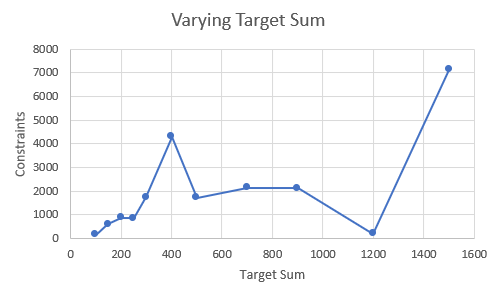
\includegraphics[width=0.8\textwidth]{graph_sum_consts.png}
    \caption{Graph for varying target sum and number of constraints}
    \label{graphSumC}
\end{figure}

\end{document}
